\section*{Sinnesorgane}

\paragraph{Geruchssinn}
\begin{itemize}
  \item \textbf{Nase}: Atmung (Reinigung + Filterung) + Geruchswahrnehmung
  \item \textbf{Geruchswahrnehmung}:
  \begin{itemize}
    \item komplexer chemisch-neuraler Vorgang
    \item Riechschleimhaut: Luft scheidet Geruchsmoleküle an Rezeptormoleküle ab
    \item Auf einzelne Duftstoffe ansprechende Rezeptoren (>350 Rezeptortypen) bilden durch Riechköpfchen Matrixstruktur an Oberfläche der Riechschleimhaut
    \item Vereinigung Duftmolekül + Rezeptor \( \to \) Kaskade in Rezeptorzellen \( \to \) neuronale Signale über Riechnerv-Axone an Großhirn
    \item Olfaktorisches System hochkomplex, Verbindungen zu Hypothalamus (Nahrungsaufnahme + Sexualverhalten) und limbischem System (Instinktverhalten + Gedächtnisleistungen)
  \end{itemize}
\end{itemize}

\paragraph{Geschmackssinn}
\begin{itemize}
  \item 5 Grundqualitäten:
  \begin{enumerate}
    \item \textbf{Süß}: Zucker + Derivate, Aminosäuren, Peptide, Alkohole
    \item \textbf{Salzig}: Speise- + Mineralsalze
    \item \textbf{Sauer}: saure Lösungen, organische Säuren
    \item \textbf{Bitter}: Bitterstoffe, Alkaloide, Glycoside (Chinin, Wermut)
    \item \textbf{Umami}: Glutaminsäure, Asparaginsäure
    \item[!] Scharf kein Geschmack, sondern Schmerzsignal
  \end{enumerate}
  \item \textbf{Primärer gustatorischer Cortex} (Inselcortex): für Geschmacks\-wahr\-nehm\-ung zuständige Hirnstruktur, mit anderen Sinneseindrücken (z.B. Tast- und Temperaturinformationen) aus Mundhöhle integriert
  \item \textbf{Sekundärer gustatorischer Cortex}: in orbito-frontalem Cortex (überlappt mit sekundären olfaktorischem Cortex)
\end{itemize}

\paragraph{Visuelle Wahrnehmung --- Auge}
\begin{figure}[H]
  \centering
  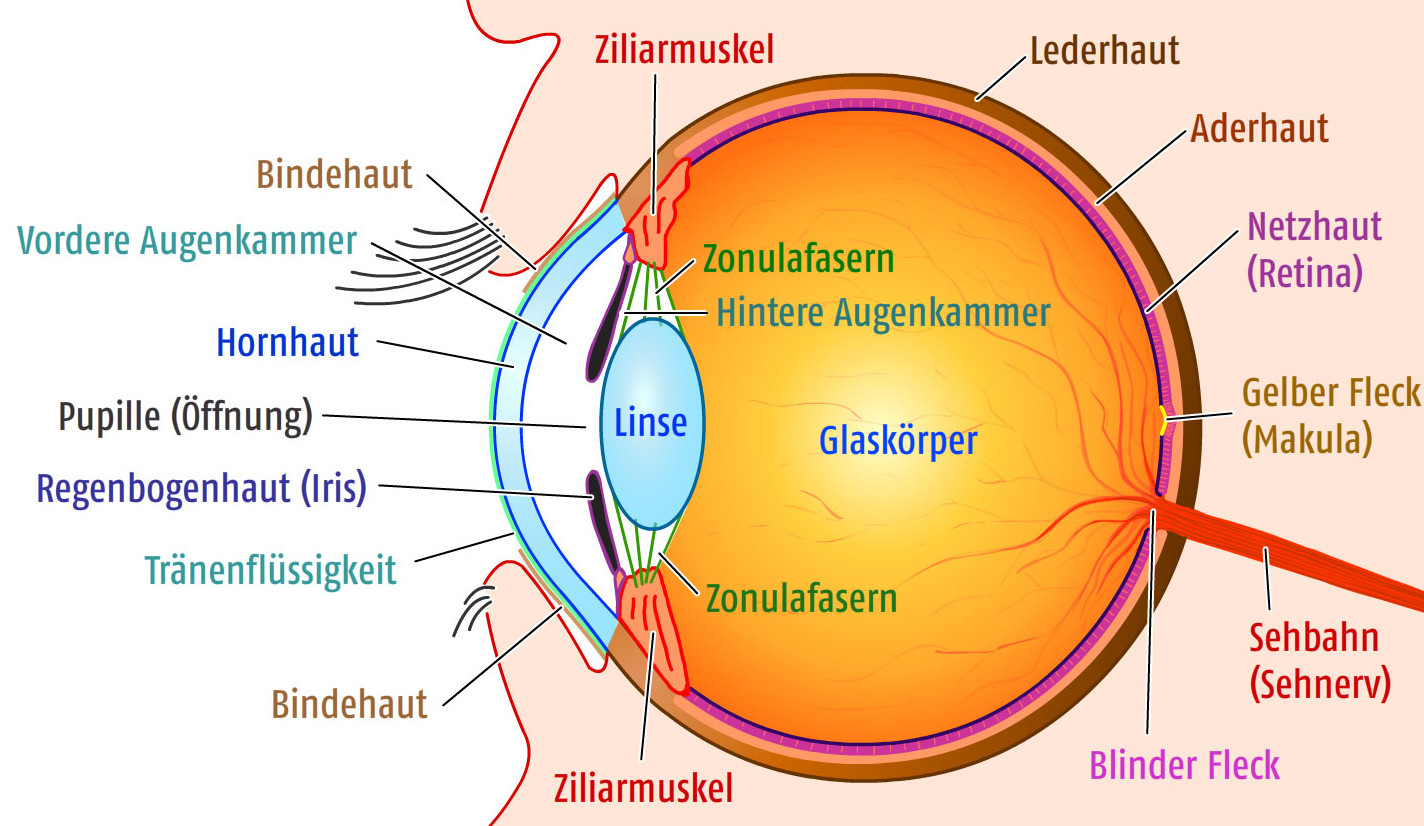
\includegraphics[width=.7\linewidth]{assets/img/auge.jpg}
\end{figure}
\begin{itemize}
  \item \textbf{Augapfel}: kugelförmig, kardanische Aufhängung \( \to \) beliebig drehbar
  \item Auge besteht aus drei Schichten:
  \begin{enumerate}
    \item \textbf{Äußere Augenhaut}:
    \begin{itemize}
      \item Durchsichtige Hornhaut (\emph{cornea}) dort, wo Licht ins Auge tritt
      \item Geht über in weiße Lederhaut (\emph{sclera}), größter Teil der Augapfelhülle --- teils von Bindehaut bedeckt, nur Cornea wird direkt von Tränenflüssigkeit benetzt
      \item Tränenflüssigkeit: fließt von Tränendrüse über \emph{canaliculi licrimales superior} und \emph{inferior} (oberer + unterer Tränenkanal) in Nasenhöhle ab
    \end{itemize}
    \item \textbf{Mittlere Augenhaut} \emph{uvea}:
    \begin{itemize}
      \item hinten gut durchblutete Aderhaut \( \to \) Nährstoffversorgung
      \item Übergang zu Ziliarkörper (\emph{corpus ciliare}) \( \to \) Aufhängung Augenlinse
      \item vorne Regenbogenhaut (\emph{iris}) + Pupille \( \to \) Regulierung Lichteinfall
    \end{itemize}
    \item \textbf{Innere Augenhaut}:
    \begin{itemize}
      \item Netzhaut + Retina, enthält Lichtsinneszellen (Photorezeptoren)
      \item Blinder Fleck dort, wo Sehnerv das Auge verlässt (Sehnervenpapille)
      \item Gelber Fleck (\emph{fovea}): Stelle des schärfsten Sehens
    \end{itemize}
  \end{enumerate}
  \item \textbf{Sensorzellen} in Retina:
  \begin{itemize}
    \item Stäbchen: Lichtsensoren (Hell-Dunkel-Unterscheidung), im peripheren Bereich
    \item Zäpfchen: Farbsensoren (3 Gruppen, violett-grün-gelb), im Fovea-Bereich
  \end{itemize}
\end{itemize}

\paragraph{Visuelle Wahrnehmung --- Weiterleitung zum Hirn}
\begin{itemize}
  \item Zäpfchen + Stäbchen ergänzt durch Rezeptoren, an welche spezielles G-Pro\-tein gebunden ist (bestehen aus Bestandteilen von Vitamin A + Opsin-Protein)
  \item \textbf{Ablauf}:
  \begin{enumerate}
    \item Eintreffende Photonen lösen in Vitamin A Strukturveränderung aus \\* \( \to \) Opsin kann mit Vitamin A agieren, Enzym-Ausschüttung
    \item Negative Ladung in Zellmembran \( \Rightarrow \) optisches zu elektrischem Signal
    \item Auswertezellen in Netzhaut: verarbeiten elektrisches Signal
    \item Weiterleitung Ganglienzellen, Fortsätze bilden II.\ Hirnnerv (\emph{nervus opticus})
  \end{enumerate}
\end{itemize}

\paragraph{Visuelle Wahrnehmung --- Visuelles System}
\begin{figure}[H]
  \centering
  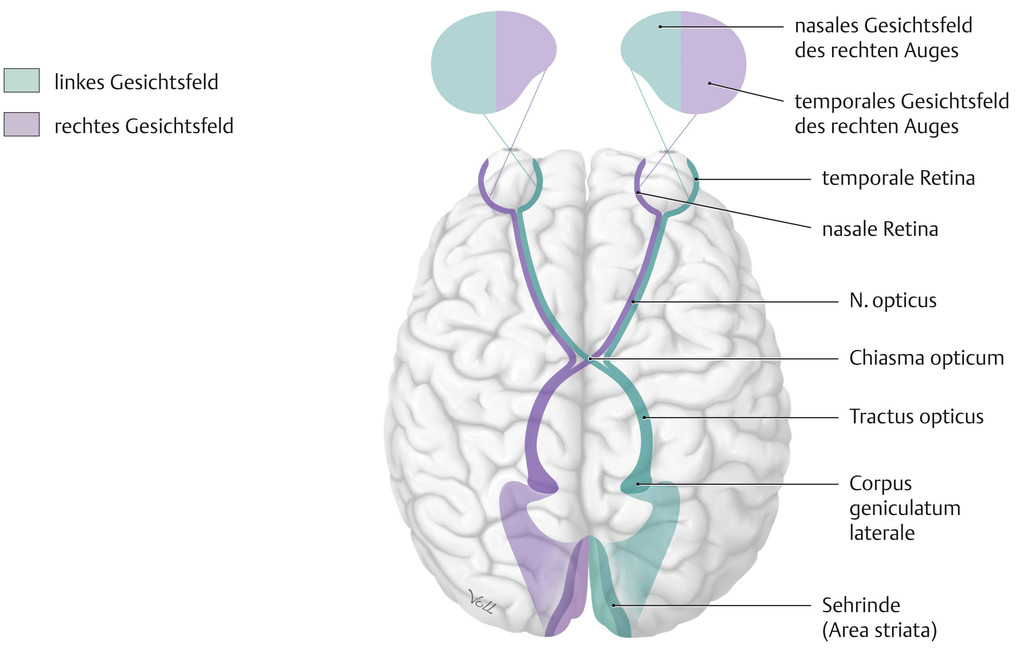
\includegraphics[width=.7\linewidth]{assets/img/visuellesSystem.jpg}
\end{figure}
\begin{itemize}
  \item \textbf{Sehrinde}: Empfängt elektrische Impulse über Sehbahnen
  \item \textbf{Sehnervenkreuzung} (\emph{chiasma opticum}): Hier kreuzen sich nach Eintritt in Schädelhöhle die Sehnerven der beiden Augen
  \item Äußere Fasern verlaufen weiter, Innere kreuzen zur Gegenseite \\* \( \to \) Fasern linke Netzhauthälfte beider Augen in linke Hirnhälfte, rechte analog
  \item \emph{\textbf{Tractus opticus}}: Weiterleitung Nervenfasern zu \textbf{seitlichen Kniehöckern} (\emph{corpus geniculatum laterale})
  \item breite Fächerung der Sehstrahlung hin zur \textbf{Sehrinde} (visueller Cortex)
\end{itemize}

\paragraph{Gehörsinn --- Ohr}
\begin{figure}[H]
  \centering
  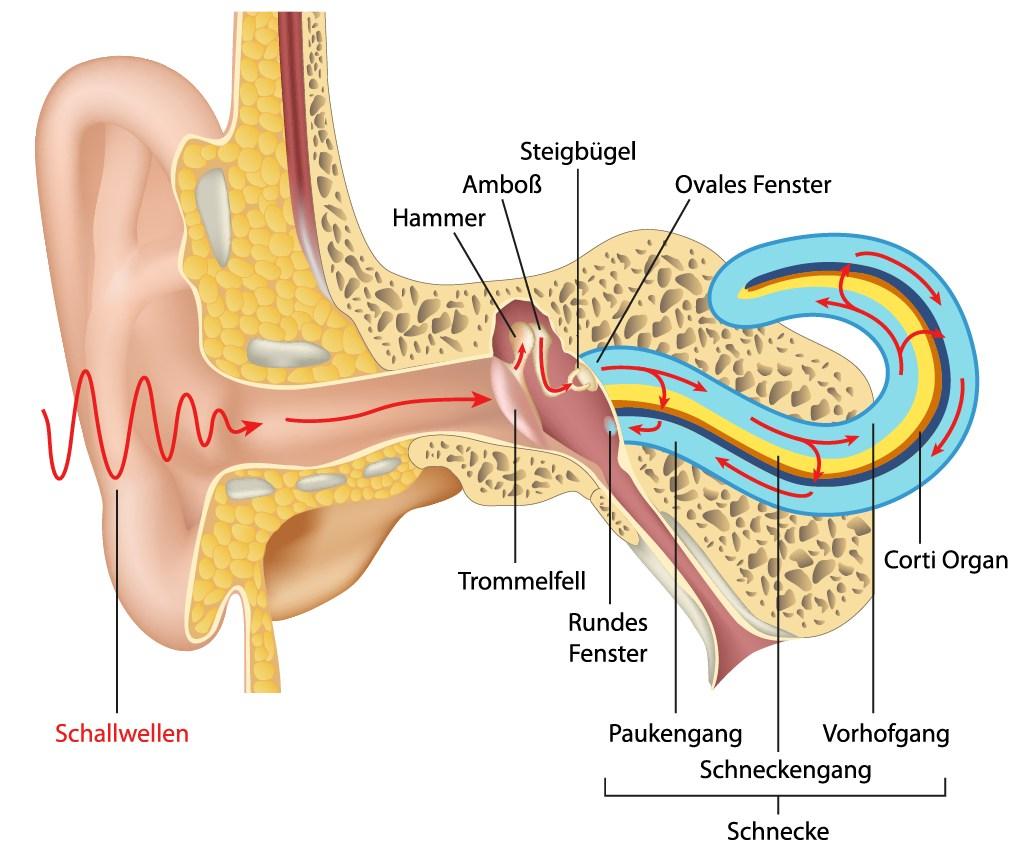
\includegraphics[width=.585\linewidth]{assets/img/ohr.jpg}
\end{figure}
\begin{itemize}
  \item \textbf{Äußeres Ohr} (Ohrmuschel, Ohrknorpel, äußerer Gehörgang): Einfangen von Schall, Codieren der Einfallsrichtung
  \item \textbf{Mittelohr} (Trommelfell, Gehörknöchelchen, Eustachische Röhre): Mechanische Impedanzwandlung \( \to \) optimale Übertragung Außenohr-Innenohr
  \item \textbf{Innenohr} (Labyrinth: Gehörschnecke (\emph{cochlea}), Bogengänge, Hörnerv): Gehörschnecke setzt Schall in Nervenimpulse um, Innenohr beherbergt Gleichgewichtsorgan (besteht aus drei Bogengängen + zwei Aussackungen (\emph{utriculus}, \emph{sacculus}))
  \item Steigbügel = Übertragungselement zur Gehörschnecke
  \item Schwingungen erregen Haarzellen in Cochlea, welche mit Hörnerv verbunden sind \( \to \) Ausschüttung Neurotransmitter \( \to \) Weiterleitung ans Gehirn
\end{itemize}

\paragraph{Gehörsinn --- Cochlea + Einortstheorie}
\begin{itemize}
  \item Frequenzabhängiges Schwingungsmaximum zw. Steigbügel und \emph{helicotrema}
  \item Hohe Frequenz \( \to \) nah bei Steigbügel, tiefe Frequenz \( \to \) nah bei Helicotrema
  \item Anregung Sinneszellen bei Maximum \( \to \) erregte Zellen frequenzabhängig
  \item[\( \to \)] Konstante Töne weniger angenehm als variierende
\end{itemize}

\paragraph{Gehörsinn --- Auditives Wahrnehmen}
\begin{itemize}
  \item \textbf{Auditiver Cortex}: Auditorische Fasern rückverschaltet \( \to \) Impulse beider Ohren kommen in beiden auditiven Cortices an \\* \( \to \) Richtungshören, Resthörempfinden bei Schäden
  \item \textbf{Oberer Olivenkomplex}: Rücksendung von Fasern zum Innenohr \\* \( \to \) Empfindlichkeitsmodulierung
\end{itemize}

\paragraph{Gehörsinn --- Gleichgewichtssinn}
\begin{figure}[H]
  \centering
  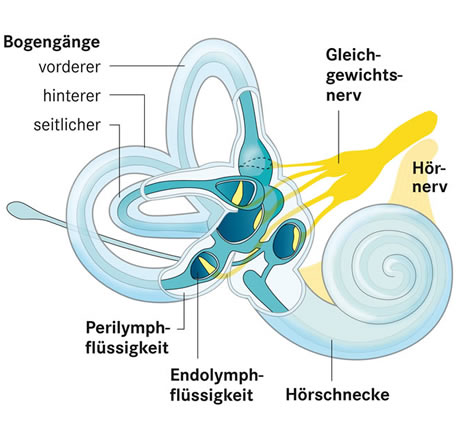
\includegraphics[width=.4\linewidth]{assets/img/gleichgewichtsorgan.jpg}
\end{figure}
\begin{itemize}
  \item \textbf{Utriculus + Sacculus}: besitzen von Gallertmasse umhüllte Sinneshaarzellen
  \item \textbf{Calciumkarbonatkristalle} auf Sinneshaarzellen, umgeben von weniger dichter Flüssigkeit
  \item Translationsbewegung \( \to \) Kristalle hinken gegenüber Bewegung nach \\* \( \to \) Beugung + Reizung Sinneshaarzellen
  \item Rotatorische Bewegungen: Ermittlung durch 3 Bogengänge
  \item Signale über VIII.\ Hirnnerv in Vestibularis-Kerne im Stammhirn weitergeleitet
  \item Nutzung zusätzlicher Informationen von Augen, Kopf und Körperstellung zur eindeutigen Lagebestimmung
\end{itemize}